\chapter{Optimización non convexa sen restriccións}
\label{sec:optimizacion}

\begin{figure}[h]
  \centering
  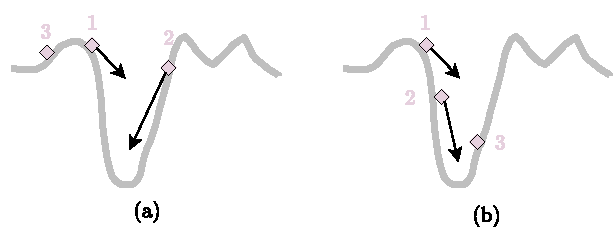
\includegraphics[width=\textwidth]{imaxes/introducion/optimizacion.drawio.pdf}
	\caption[Ilustración da influencia da eleción da tasa de aprendizaxe. Figura de autoría propia.]{Ilustración da influencia da eleción da tasa de aprendizaxe. Repórtase un un punto incicial ($1$) co seu gradiente negativo (dirección de máximo descenso), e as dúas iteracións seguintes. En (a) empregouse unha tasa de aprendizaxe grande que supón trucar de ``parede'' en cal de avanzar nunha dirección. En (b) utilizouse unha tasa de aprendizaxe máis baixa o que permite seguir na mesma rexión polo menos ata que se está suficientemente preto do mínimo. Figura de autoría propia.}
  \label{fig:optimizacion}
\end{figure}
\nota{falar da influencia do learning rate nos tambaleos do adestramento da Rede (para a sección \ref{sec:res-bus-rfmid}) }

\nota{falar da Figura \ref{fig:optimizacion}}

\nota{falar de que en todo o traballo usamos AdamW \cite{adamw} e que ten weigth decay. tal cosa é importante}

\nota{nalgún lugar ten que dicirse que as funcións de pérdida de a rede normal e a de segundo orde non son igual de difíciles, en particular a de segundo orde é máis difil porque como cada parémetro esta sometido a máis operación realemente ten máis restriccións. o cal nun problema sinxelo com drive axuda á converxencia pero en problemas complexos como RFMiD a dificulta.}

\nota{falar da relación converxencia - dimensión VC (para a sección \ref{sec:res-bus-imagenet}) (ou non?)}
